\documentclass[paper=a4, parskip=half-]{scrartcl}
\usepackage[utf8]{inputenc}

\usepackage{amsmath}
\usepackage{mathtools}
\usepackage{amssymb} % more icons/symbols
\usepackage{hyperref} % for hyper links
\usepackage{graphicx}
\usepackage{enumitem} % for enumerations a), i)

\usepackage{geometry}
 \geometry{
 a4paper,
 left=20mm,
 right=20mm,
 top=20mm,
 bottom=30mm,
 }


\title{Algorithmik für Schwere Probleme}
\author{\texttt{thgoebel@ethz.ch}}
\date{ETH Zürich, FS 2021}

% Custom commands
\newcommand{\setzeroone}{\lbrace 0, 1 \rbrace} % => {0,1} (Notice the missing $$)
\newcommand{\binarystring}{\setzeroone^*}
\newcommand{\horizontaldivider}{\begin{center} \line(1,0){350} \end{center}}
\newcommand{\A}{\mathcal{A}}
\newcommand{\M}{\mathcal{M}}
\newcommand{\bigO}{\mathcal{O}}
\newcommand{\N}{\mathbb{N}}
\newcommand{\Time}{\text{time}}


\begin{document}

\begin{titlepage}
\maketitle
\vspace{5cm}
\thispagestyle{empty}


\begin{abstract}
This documents is a \textbf{short} summary for the course
\textit{Algorithmik für Schwere Probleme} at ETH Zurich.
It is intended as a document for quick lookup, e.g. during revision,
and as such does not replace attending the lecture, reading the slides or reading a proper book.

We do not guarantee correctness or completeness, nor is this document endorsed by the lecturers.
Feel free to point out any erratas.
\end{abstract}

\end{titlepage}

\tableofcontents
\newpage
%\listoffigures
%\listoftables

%Credits: images are generally taken from the lecture slides.
\newpage

\section{Einführung}

\begin{takeaway}
    \item NP-schwer vs. NP-vollständig
    \item Schwellwertsprache
\end{takeaway}

\paragraph{Polynomzeit-Reduzierbarkeit}
Ein Entscheidungsproblem $\Pi_1$ ist ``polynomzeit-reduzierbar'' auf ein anderes
Entscheidungsproblem $\Pi_2$:
\begin{align*}
& \Longleftrightarrow
\exists \text{ Algo } \A \text{ s.t. } \Time_\A \in \text{poly}
\wedge \Pi_1(x) = \Pi_2(\A(x))
\\
& \Longleftrightarrow
\Pi_2 \text{ mindestens so schwer wie } \Pi_1
\\
& \Longleftrightarrow
\Pi_1 \text{ höchstens so schwer wie } \Pi_2
\\
& \Longleftrightarrow
\Pi_1 \preceq_P \Pi_2
\end{align*}

\paragraph{NP-schwer (NP-hard)}
Ein Problem $\Pi$ das ``mindestens so schwer'' ist wie alle Probleme in NP.
D.h. alle Probleme in NP lassen sich auf $\Pi$ reduzieren:
$$ \forall \Pi' \in NP : \Pi' \preceq_P \Pi $$
$\Pi$ muss nicht notwendigerweise in NP liegen (d.h. kann schwerer sein)!
Beispiel: das Halteproblem (nicht entscheidbar, daher $\notin NP$).

\paragraph{NP-vollständig (NP-complete)}
Ein Problem $\Pi$, das in NP liegt \underline{und} NP-schwer ist.
``Repräsentativ'' für die Menge NP, da sich alle Probleme aus NP darauf reduzieren lassen. \\
Beispiel: Satisfiability-Problem SAT (Satz von Cook).

\begin{figure}[h]
    \centering
	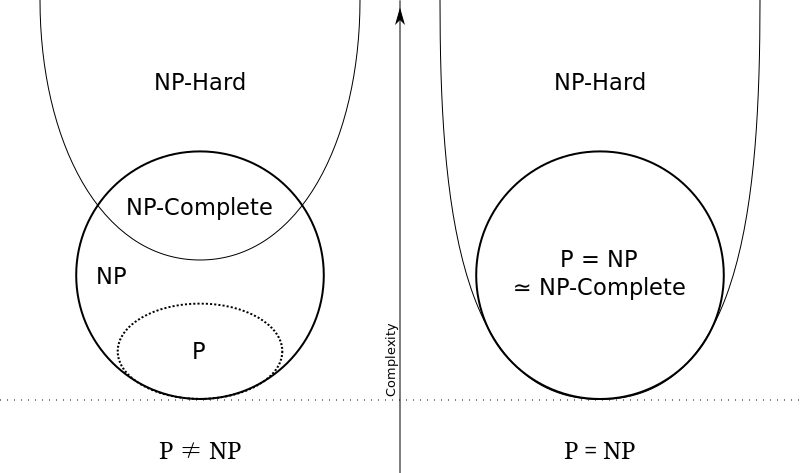
\includegraphics[scale=0.4]{images/np-hard-complete.png}
    \caption{Mengendiagramm der Beziehungen (Quelle: \href{https://commons.wikimedia.org/w/index.php?curid=3532181}{Wikipedia})}
    \label{fig:pke-ind-cca}
\end{figure}

\paragraph{``Schwere Probleme''}
NP-schwere Probleme, aber generell alle Probleme die sich nicht in Polynomzeit lösen lassen.
\textbf{Sinnvollerweise gehen wir im Folgenden davon aus dass $P \neq NP$.}

Alle Instanzen unseres Problems sind deterministisch in Polynomzeit \underline{nicht} lösbar.
Mögliche Ansätze:
\begin{enumerate}[label=\alph*)]
    \item nicht exakt sondern approximativ lösen (Approximationsalgorithmen)
    \item nicht deterministisch sondern nichtdeterministisch lösen (Randomisierte Algorithmen)
    \item nicht polynomiell sondern moderat exponentiell lösen%
    \footnote{D.h. die Basis der Exponentation ist klein, z.B. $1.4^n$ statt $2^n$.}
    \item nicht alle sondern alle Instanzen mit einer bestimmten Struktur lösen (Parametrisierte Algorithmen)
    \item anderweitig zusätzliche Informationen über die Eingabe nutzen (Reoptimierung, Win-Win-Strategy)
    \item Heuristiken\footnote{Nachteil: Im Gegensatz zu den anderen Ansätzen ist hier die Qualität (Laufzeit, ...) nicht beweisbar.}
\end{enumerate}


\subsection{Definitionen}

\paragraph{Entscheidungsproblem}
$P = (L, U, \Sigma)$ wobei
\begin{itemize}
    \item $\Sigma$ ein Alphabet
    \item $U \subseteq \Sigma^*$ die Menge der zulässigen Eingaben (als Wörter über dem Alphabet, als \emph{Sprache})
    \item $L \subseteq U$ die Menge der akzeptierten Eingaben (\emph{JA-Instanzen})
\end{itemize}
Ein Algorithmus $\A$ \emph{löst} $P$ falls gilt:
$$ \forall u \in U : A(x) =
\begin{cases}
1 \text{ oder JA}, \text{ if } x \in L \\
0 \text{ oder NEIN}, \text{ if } x \in U-L \\
\end{cases}
$$

\paragraph{Vertex Cover Problem VC}
``Der Hefepilz der parametrisierten Algorithmiker -- ein Modellproblem.''
\\
Eingabe $U$: ungerichteter Graph $G = (V, E)$ und $k \leq |V|, k \in \N$. \\
Ausgabe $L$: JA falls $\exists C \subseteq V$ s.t. $|C| \leq k$ mit $\forall \{u, v \} \in E: u \in C \vee v \in V$.

\paragraph{Satisfiability-Problem SAT} \mbox{} \\
Eingabe: CNF-Formel $\Phi = C_1 \wedge \dots \wedge C_m$ mit Klauseln $C_i$ über Variablen $x_1, \dots, x_n$. \\
Ausgabe: eine Variablen-Belegung die $\Phi$ erfüllt.

Bei $l$-SAT enthält jede Klausel maximal $l$ Literale.

\paragraph{Optimierungsproblem}
$U = (L, M, cost, goal)$ wobei
\begin{itemize}
    \item $L$ die Sprache der zulässigen Eingaben\footnote{Oben noch $U$!}
    \item $\M: L \mapsto \Sigma^*$ so dass $M(x)$ die Sprache der akzeptierten Lösungen für Eingabe $x$
    \item $cost$: $\forall x \in L \; \forall y \in M(x) : cost(y, x) = $ Kosten der Lösung $y$ für Eingabe $x$
    \item $goal \in \{ \min, \max \}$ das Optimierungsziel
    \item $Opt_U(x) = goal \{ cost(y, x) | y \in M(x) \}$ die Kosten einer optimalen Lösung für Eingabe $x$
\end{itemize}

\paragraph{Minimum Vertex Cover Problem MIN-VC}
Wie VC, mit $cost(C, G) = |C| = $ Grösse des Vertex Covers und $goal = \min$.

\paragraph{MAX-SAT}
Wie SAT, mit $cost = $ Anzahl belegte Variablen und $goal = \max$.

\paragraph{Laufzeit}
eines Algorithmus' $\A$ auf Eingabe $x$ ist $\Time_\A (x)$
wobei $\Time_\A: \N \mapsto \N$.
Die Laufzeit von $\A$ in Abhängigkeit von der Grösse $n$ der Eingabe ist:
$\Time_\A (n) = \max \{ \Time_\A (x) \; | \; |x| = n, x \in L \}$.
Die Laufzeit wird in  $\bigO$-Notation angegeben.

\paragraph{Schwellwertsprache (threshold language)} definiert für ein Optimierungsproblem $U$:
$$ Lang_U = \{ (x, a) \in L \times \binarystring \; | \; Opt_U(x) \leq Number(a) \} $$
wo $Number(a)$ die Zahl mit der Binärdarstellung $a$ (der \emph{Schwellwert}) ist und $goal = \min$.
\\
Beispiel: $Lang_{MIN-VC} = VC$. Aber $Lang_{MAX-SAT} \neq SAT$ (da SAT leichter sein kann)!

$U$ heisst ``NP-schwer'' falls $Lang_U$ NP-schwer ist (warum?).%
\footnote{Recall that NP-Schwere für Entscheidungsprobleme definiert ist.
Über die Schwellwertsprache erweitern wir dies für Optimierungsprobleme.}

\newpage

\section{Pseudopolynomielle Algorithmen}

\begin{takeaway}
    \item Pseudopolynomialität
    \item Stark NP-schwer
\end{takeaway}

\paragraph{Zahlproblem (integer value problem IVP)} 
Probleme, dessen Eingaben vollständig durch Integer darstellbar sind.

Eingabe $x = x_1 \# \dots \# x_n \; ; \; x_i \in \binarystring$, interpretiert 
als Vektor $\text{int}(x) = (\text{number}(x_i), \dots, \text{number}(x_n))$.

Weiter sei 
\[\text{max-int}(x) = \max_{i \in \{1, ..., n\}} \text{number}(x_i)\]
die grösste vorkommende Zahl (im Wert, nicht in der Darstellung). Da die 
Eingabe binär definiert ist, kann $Max-Int(x)$ exponentiell in $|x|$ sein.

\textbf{Beispiel:} Travelling Salesperson Problem TSP (via Adjazenzmatrix des Graphen).

\paragraph{Pseudopolynomiell}
Sei $U$ ein Zahlproblem und $\A$ ein Algorithmus der $U$ löst.
$\A$ heisst \emph{pseudopolynomiell} falls für alle Eingaben $x$ ein 
Polynom $p$ existiert, so dass 
\[ \Time_\A (x) \in \bigO \Big( p \big( |x| , \text{max-int}(x) \big) \Big)\]
D.h. auf Eingaben mit ``kleinen Zahlen'' ist $\A$ polynomiell.

\paragraph{h-beschränktes Teilproblem}
Sei $U$ ein Zahlproblem, $h: \N \mapsto \N$ monoton nicht-fallend.
Das \emph{h-beschränkte Teilproblem von $U$ (h-value-bounded subproblem)} 
$\text{value}(h)\text{-}U$ ist das Teilproblem mit Eingaben $I$ für 
die gilt: $\text{max-int}(I) \leq h(|I|)$.

\paragraph{Stark NP-schwer}
Ein Zahlproblem $U$ heisst \emph{stark NP-schwer} falls ein Polynom $p$ existiert, 
so dass $\text{value}(p)\text{-}U$ NP-schwer ist.

In anderen Worten: $U$ ist stark NP-schwer wenn es auch dann NP-schwer ist wenn 
alle darin vorkommenden Zahlen ``klein'' sind.

Beispiel: TSP ist stark NP-schwer. Generell jedes gewichtete 
Graph-Optimierungsproblem ist NP-schwer, wenn das ungewichtete Pendant 
NP-schwer ist (bei TSP also das Hamiltonkreisproblem HCP).

\paragraph{Theorem}
Sei $U$ stark NP-schwer. Dann existiert kein pseudopolynomieller Algorithmus für $U$. 
\footnote{Wie immer unter der Annahme dass $P \neq NP$.}

Beweis Ansatz: Wir nehmen an, dass ein pseudo poly. Algorithmus $\mathcal{A}$ 
für $U$ existiert. Über die Definition von Stark NP-schwer können wir dann 
zeigen, dass wir ein polynomiellen Algorithmus für $\text{value}(p)\text{-}U$ 
hätten, was ein Widerspruch ist.


\subsection{Rucksackproblem (Knapsack problem, KP)}\label{algo-kp}

\paragraph{Rucksackproblem}
Wie viel Diebesgut kann ich mitnehmen.

\textbf{Eingabe $I$:} Gewichte $w_i \in \N^+$, Kosten/Nutzen $c_i \in \N^+$, 
Limit/Kapazität $b \in \N^+$, wo $i \in \{ 1, \dots, n \} $. \\
\textbf{Ausgabe:} Indexmenge $T \subseteq \{ 1, \dots, n \}$ s.t. $\sum_{i \in T } \leq b$ \\
\textbf{Kosten:} $cost(T, I) = \sum_{i \in T} c_i$ \\
\textbf{Ziel:} $\max$

\paragraph{Lösung mit Dynamischer Programmierung (Dyn-Prog-KP)} 
Wir iterieren über alle Teilprobleme $I_i$ und speichern die Tripel
$(k, W_{i, k}, T_{i, k})$ = (Nutzen, Gewicht, Indexmenge), also Mengen $T_{i, k}$
die exakt Nutzen $k$ mit minimalen Gewicht $W_{i, k}$ erreichen.
In jeder Iteration behalte für jeden vorhandenen Nutzen ein Tripel mit minimalen Gewicht.
Lese am Ende den maximal erreichten Nutzen $k^*$ (und sein $T_{n, k^*}$) aus.

\paragraph{Laufzeit} \[\bigO \big( |I|^2 \cdot \text{max-int}(I) \big)\] da der 
Algorithmus $|I|$ Iterationen durchläuft und
jeder Schritt in $\leq \sum_j^n c_j = |I| \cdot \text{max-int}(I)$ läuft.

\paragraph{Verbesserung falls \(b \ll \sum_{j=i}^{n} c_j\):}
Wir können den Algorithmus für Instanzen verbessern, 
bei denen die Gewichtsschranke kleiner ist als die Summe aller Nutzen.

Im oben stehenden Algorithmus speichern wir uns ein Tripel für jeden möglichen 
Nutzen (es gibt \(\sum_{j=i}^{n} c_j\) solche Werte) das minimal Gewicht (und 
die jeweiligen Gegenstände), das diesen Nutzen erreicht. Da \(b \ll \sum_{j=i}^{n} c_j\) 
können wir die Logik des Algorithmus ``umkehren'' und stattdessen für jedes 
mögliche Gewicht den maximal erreichbaren Nutzen speichern. 

Die neue Laufzeit des neuen Algorithmus ist in \(\bigO \left (n \cdot b\right)\), 
wobei \(n \in \bigO(|I|)\) und \(b \in \bigO(\text{max-int}(I))\).

\paragraph{Weitere Verbesserung} Wir können die zwei Ansätze kombinieren für 
Probleme bei denen \(b \gg \sum_{j=i}^{n} c_j\), wobei allerdings nur wenig 
Objekte die Summe stark beeinflussen. Also wir nehmen an es gibt ein \(i \ll n\), 
sodass \(b \gg \sum_{j=i}^{n - i} c_j\) und \(b \ll \sum_{j=i}^{n} c_j\).

Hierfür unterteilen wir das Problem in zwei Teilprobleme, eines, was nur die 
``leichten'' Objekte enthält und eines welches nur die ``schwere'' Objekte beinhaltet. 
Wir rufen den ursprünglichen Algorithmus auf der ``leichten Instanz''\footnote{Leichte 
Instanz im Sinne von Gewicht, nicht Komplexität} auf und die oben beschriebene 
Verbesserung auf die ``schwere Instanz''. Wir können die beiden Lösungen nun kombinieren, 
indem wir für jede Lösung des einen Problems, die best mögliche Lösung aus dem anderen 
Problem suchen. Die Lösung ist die Kombination mit dem höchsten Gesamtnutzen.

Die Laufzeit des Algorithmus ist in
\[\bigO\left(n \cdot \sum_{j = 1}^{n-i} + i \cdot b \right).\]

\newpage

\section{Parametrisierte Algorithmen}

\begin{takeaway}
    \item Parametrisierter Algorithmus, fpt
    \item Standard-Parametrisierung
    \item Kernbildung
\end{takeaway}

\paragraph{Idee}
Verallgemeinerung von pseudopolynomiellen Algorithmen:
Laufzeit hängt von der Eingabegrösse nur polynomiell ab, aber darf extrem gross werden in der Grösse eines Parameters.
Partitionierung in Problemklassen entlang des Parameters.

\paragraph{Parametrisierung}
Sei $U$ ein Entscheidungsproblem, $L$ die Sprache der Eingaben.
$\Par: L \mapsto \N$ ist eine \emph{Parametrisierung} von $U$ falls gilt:
\begin{enumerate}[label=(\roman*)]
    \item $\Par$ ist in Polynomzeit berechenbar
    \item Für unendlich viele $k \in \N$ ist die Parameter-$k$-Menge für $U$
    $$ Set_U(k) := \{ I \in L \st \Par(I) = k \} $$ unendlich.
    Dies stellt sich dass $\Par$ nichttrivial ist, z.B. nicht etwa $\Par(I) = |I|$.
    In anderen Worten, für jeden Parameterwert soll es beliebig viele Probleminstanzen geben.
\end{enumerate}
Ein Algorithmus $\A$ heisst \emph{$\Par$-paremetrisierter Polynomzeit-Algorithmus} für $U$ falls gilt:
\begin{enumerate}[label=(\roman*)]
    \item $\A$ löst $U$
    \item $ \exists \text{ Polynom } p \; \exists \text{ (berechenbare) Funktion } f : \N \mapsto \N$
    so dass $\forall I \in L$:
    $$\Time_\A(I) \leq f \big( \Par(I) \big) \cdot p(|I|) $$
\end{enumerate}
Dann heisst $U$ \emph{fixed-parameter-tractable bezüglich $\Par$}.
$\A$ heisst auch \emph{fpt-Algorithmus für $U$ bezüglich $\Par$} und läuft in fpt-Zeit.

\underline{Beispiel:}
Sei $U$ ein Zahlproblem und sei $Val(I) := \max \{ |x_i| \}$.
Es gilt $Max-Int(I) \leq 2^{Val(I)}$ und ist $Val$ eine Parametrisierung von $U$.

\paragraph{Ansätze}
Die \emph{Standard-Parametrisierung} wählt als Parameter die Grösse der gewünschten Lösung (z.B. Grösse des VCs).
Die \emph{Strukturelle Parametrisierung} wählt eine bestimmte Eigenschaft der Eingabe (z.B. maximaler Knotengrad).
Andere Ansätze betrachten wir im Folgenden.


\subsection{Kernbildung}

\paragraph{Idee}
Polynomielles Preprocessing, Datenreduktion, um die Instanz auf einen \emph{Kern} zu verkleinern,
der in seiner Grösse nur noch vom Parameter abhängt.
Diesen Kern dann mit bekannten Algorithmen (oder brute force) lösen.

\paragraph{Kernbildung (kernelisation)}
Sei $(U, \Par)$ ein parametrisiertes Entscheidungsproblem, $L$ die Sprache der JA-Instanzen von $U$.
Ein \emph{Kernbildungs-Algorithmus} für $(U, \Par)$ ist ein Polynomzeit-Algorithmus $\A$ der jede Eingabe $(I, k)$
in eine neue Eingabe $(I', k')$ (den \emph{Kern (kernel)}) transformiert so dass:
\begin{enumerate}[label=(\roman*)]
    \item $ I \in L \iff I' \in L $ (Korrektheit)
    \item $ |I'| + k' \leq g(k) $ für $g : \N \mapsto \N$ (neue Grösse nur abhängig vom alten Parameterwert $k$)
\end{enumerate}

\paragraph{Beispiel: VCP} \mbox{} \\
\underline{Reduktionsregel:}
Sei $S \subseteq V$ ein VC von $G$ so dass $|S| \leq k$. Dann enthält $S$ alle Knoten mit $\deg_G(v) > k$ (warum?).
Dann gilt für ein solches $v$:
$$ (G, k) \in VCP \iff (G-\{v\}, k-1) \in VCP $$
Zusätzlich entferne alle isolierten Knoten mit $\deg_G(v) = 0$ (sie decken keine Kanten ab).

Zu zeigen: wenn die Regel nicht mehr anwendbar ist, dann hat der verbleibende Graph $G'$ entweder kein vertex cover,
oder aber er ist ``klein genug'' (nur noch anhängig von $k$), also ein Kern.

\underline{Beobachtung:}
Sei $G$ ein Graph ohne isolierten Knoten, mit einem vertex cover der Grösse $m$ und mit $\max \deg_G(v) \leq k$.
Dann gilt $|V| \leq m \cdot (k+1)$ (warum?).%
\footnote{Falls $|V| > k \cdot (k+1)$, dann wir wissen dass $ I \notin L$ und können NEIN ausgeben.}

\underline{Theorem:}
Diese Reduktionsregeln berechnen einen Kern der Grösse $\bigO (k^2)$ in Zeit $\bigO (k \cdot n)$.

\underline{Parametrisierter Algorithmus:}
Berechne einen Kern $(G', k')$. Wenn der Kern zu gross ist, geben NEIN aus.
Andernfalls prüfe durch vollständige Suche ob ein VC mit $|S'| \leq k'$ existiert.

\underline{Theorem:}
Dies ist ein fpt-Algorithmus bzgl. der Standard-Parametrisierung. Die Laufzeit beträgt
$\bigO (k \cdot n + k^{2k+2}) \subseteq \bigO (k^{2k+2} \cdot n)$.


\subsection{Suchbäume}


\subsection{Iterative Kompression}



\newpage

\end{document}
